\chapter{High-rate motion data pre-integration}
\label{chp:pre-integration}
\minitoc
\bigskip


Sensor modalities available on robotic platforms display a great variety in the rate at which measurements are acquired. For instance, 
a camera may record images at 33Hz while an IMU may be updated at 1kHz. In the context of Factor Graph estimation, this creates a challenge since residuals
are defined between \keyframes\ selected at a relatively low frequency, at times as low as 1Hz. One needs to integrate measurements from these high-rate sensors between \keyframes,
which is not trivial in general.

In this chapter, we first describe the example of the integration of IMU measurements which motivates the development of the pre-integration theory \cite{lupton-09,forster2017-TRO}.
We then express this pre-integration in more abstract mathematical terms to generalize it to other high-rate sensors \cite{atchuthan-18-thesis}. 
Then, we describe a possible reformulation of the original IMU-pre-integration algorithm \cite{forster2017-TRO} by exploiting a new Lie group that we 
proposed in \cite{fourmy2019absolute}. We conclude the chapter with a discussion of related works.

  
\section{A motivational example: IMU integration for graph optimization}
\label{sec:imu_preint_motivation}

In this section, we will introduce the IMU measurement model and explain why a naive integration of these measurements in the world frame does not immediately
lead to a viable factor in practice. We will then introduce the observations that lead to the development of the so-called IMU pre-integration algorithm by Lupton \cite{lupton-09},
which we reformulated with what we hope to be a more systematic approach. This systematic formulation will then be used 
in the following chapters to account for force measurements.

Let us consider the estimation of a robot base state comprised of its pose and velocity in the world frame,
%
\begin{equation}
    \bfx = [\posi{W}{WB}, \vel{W}{WB}, \Rot{W}{B}]
    \triangleq 
    [\bfp, \bfv, \Rot{}{}].
\end{equation}

We make a few hypotheses. First, we neglect effects due to the rotation of the Earth by assuming 
that our world frame (which is fixed \wrt the ground) is an inertial frame. This is a common simplification in robotics scenarios \cite{forster2017-TRO}. 
Second, without loss of generality, we assume that the IMU frame is identical to the base frame in the following developments.

The IMU measurements are known to be noisy, biased, and affected by the gravity,
%
\begin{equation}
    \begin{split}
    \angvelm{}{} &= \angvel{B}{WB} + \bias_{\angvel{}{}} + \noise_{\angvel{}{}} 
    \\
    \accm{}{}    &= \acc{B}{WB} + \bias_{\acc{}{}} + \noise_{\acc{}{}} + \Rot{B}{W} \grav .
    \end{split}
    \label{eq:imu_meas_model}
\end{equation}
%    
The biases $\bias \triangleq [\bias_{\acc{}{}}, \bias_{\angvel{}{}}]$ need to be estimated in order to be able to cancel them, and are thus included in the estimator state.
Fusing with other sensors will help make them observable.

These biases may drift over time, more or less slowly depending on the quality of the IMU. This drift is modeled 
as a random walk, which is close to the observed behavior for reasonably short periods of time \cite{hussen2015low}.

A continuous-time dynamical model  based on strap-down integration of IMU measurements can then be derived:
%
\begin{align}
\begin{split}
    \dot{\posi{}{}} &= \vel{}{} \\
    \dot{\vel{}{}} &= \acc{W}{WB} \\
    \dot{\Rot{}{}} &= \Rot{}{} [\angvel{B}{WB}]_{\times} \\
    \dot{\bias}_{\bfa} &= \bfw_{\bfa}^c \\
    \dot{\bias}_{\angvel{}{}} &= \bfw_{\angvel{}{}}^c ,
\end{split}
\label{eq:imu_dyn_conti}
\end{align}
%
where $\bfw_{\bfa}^c \in \mathcal{N}(0,\bfW_\bfa^c)$ and $\bfw_{\bw}^c \in \mathcal{N}(0,\bfW_\bw^c)$ are the biases' random walk continuous-time white noises.

Introducing the measurement equations \eqRef{eq:imu_meas_model} in the continuous dynamics equations \eqRef{eq:imu_dyn_conti} and using a zero order hold
explicit Euler integration scheme during $\dt$ results in the discrete-time dynamics:
%
\begin{equation}
    \begin{split}
    \posi{}{}^{k+1} &= \posi{}{}^{k} + \vel{}{}^{k}\dt + \frac{1}{2}\grav \dt^2 
    + \frac{1}{2}\Rot{}{}^{k}(\accm{}{}^k - \bias_{\acc{}{}}^k - \noise_{\acc{}{}}^k)\dt^2 \\
    \vel{}{}^{k+1}  &= \vel{}{}^{k} + \grav \dt + \Rot{}{}^{k}(\accm{}{}^k - \bias_{\acc{}{}}^k - \noise_{\acc{}{}}^k)\dt
    \\
    \Rot{}{}^{k+1}  &= \Rot{}{}^{k}\Exp((\angvelm{}{}^k - \bias_{\angvel{}{}}^k - \noise_{\angvel{}{}}^k)\dt)
    \\
    \bfb_\bfa^{k+1} &= \bfb_\bfa^k + \bfw_\bfa\\
    \bfb_{\angvel{}{}}^{k+1} &= \bfb_{\angvel{}{}}^k + \bfw_{\angvel{}{}}
    \end{split}
    \label{eq:imu_dyn_disc}
\end{equation}
%
where $\bfw_{\bfa} \in \mathcal{N}(0,\bfW_\bfa)$ and $\bfw_{\bw} \in \mathcal{N}(0,\bfW_\bw)$ are the bias' random walk discrete-time white noises, 
satisfying $\bfW_\bfa=\bfW_\bfa^c \dt$ and $\bfW_\bw=\bfW_\bw^c\dt$.

    
Now, these equations relate consecutive states with data sampled at IMU frequency. To include these measurements in our smoothing estimator,
one solution would be to introduce new states at the rate of the IMU. However, the size of the problem would grow very quickly due to the high acquisition rate of IMUs. 
A better option is to integrate IMU measurements during extended periods, that is between \keyframes. 
If we simply integrate the sequence of IMU measurements $\cZ_{im}$ between timestamps 
$t_i$ and $t_m$ by recursively applying \eqRef{eq:imu_dyn_disc}, we obtain:
%
\begin{equation}
    \begin{split}
    \posi{}{}^{m} &= \posi{}{}^{i} + \sum_{k=i}^{m} \Big[\vel{}{}^{k}\dt + \frac{1}{2}\grav \dt^2 
    + \frac{1}{2}\Rot{}{}^{k}(\accm{}{}^k - \bias_{\acc{}{}}^k - \noise_{\acc{}{}}^k)\dt^2 \Big] \\
    \vel{}{}^{m}  &= \vel{}{}^{i} + \sum_{k=i}^{m} \Big[\grav \dt + \Rot{}{}^{k}(\accm{}{}^k - \bias_{\acc{}{}}^k - \noise_{\acc{}{}}^k)\dt \Big]  \\
    \Rot{}{}^{m}  &= \Rot{}{}^{i} \prod_{k=i}^{m} \Exp((\angvelm{}{}^k - \bias_{\angvel{}{}}^k - \noise_{\angvel{}{}}^k)\dt) 
    \end{split}
    \label{eq:imu_int_world}
\end{equation}
%
where we assume that IMU biases stay constant during $\Dt_{im}$
\begin{equation*}
    \bias^k \approx \bias^i  ~~~ \forall k \in [i..m],
\end{equation*}
%
which makes their integration trivial and thus allows us to concentrate in the upper three lines of the model.




We are here in the position of illustrating why a naive definition of data integration leads to very bad performance. 
By observing \eqRef{eq:imu_int_world} we can define a motion error, as follows. 
First, we naively define the motion increments or "deltas"
%
% \begin{equation}
%     \D_{im} = \left[\Dp_{im}, \Dv_{im}, \DR_{im} \right] \quad , \quad (\Dp_{im},\Dv_{im},\DR_{im}) \in \cM_{\D}=\left< \Reals^3,\Reals^3, \SO(3) \right>
%     \label{eq:delta_imu_def}
% \end{equation}
%
in two ways. 
%Note that delta quantities here belong to the composite Lie group $\left< \Reals^3,\Reals^3\in \SO(3) \right>$. 
From the integration of the motion model, %we get
%
\begin{align}
    \D_{im}(\bias^i, \bfx^i) = 
    \begin{bmatrix}
    \Dp_{im}\\ \Dv_{im}\\ \DR_{im}
    \end{bmatrix} \triangleq
    \begin{bmatrix}
    \sum_{k=i}^{m} \Big[\vel{}{}^{k}\dt + \frac{1}{2}\grav \dt^2 
    + \frac{1}{2}\Rot{}{}^{k}(\accm{}{}^k - \bias_{\acc{}{}}^i)\dt^2 \Big] \\
    \sum_{k=i}^{m} \Big[\grav \dt + \Rot{}{}^{k}(\accm{}{}^k - \bias_{\acc{}{}}^i)\dt \Big]  \\
    \prod_{k=i}^{m} \Exp((\angvelm{}{}^k - \bias_{\angvel{}{}}^i)\dt)  
    \end{bmatrix}
    \label{eq:imu_delta_forster_naive}
\end{align}
%
and from the difference between initial and final states:
%
\begin{align}
    \hat\D_{im}(\bfx^i, \bfx^m) = 
    \begin{bmatrix}
    \hat\Dp_{im}\\ \hat\Dv_{im}\\ \hat\DR_{im}
    \end{bmatrix} \triangleq
    \begin{bmatrix}
    \posi{}{}^{m} - \posi{}{}^{i} \\
    \vel{}{}^{m}  - \vel{}{}^{i}  \\
    \Rot{}{}^{i,T} \Rot{}{}^{m}  
    \end{bmatrix}.
\end{align}
%
Then, we build a residual error as
%
\begin{equation}
    \bfe(\bfx_i, \bfx_m, \bias_i) 
    = \D_{im}(\bias^i, \bfx^i) \ominus \hat\D_{im}(\bfx^i, \bfx^m) =
    \begin{bmatrix}
    \Dp_{im} - \hat\Dp_{im} \\ 
    \Dv_{im} - \hat\Dv_{im} \\ 
    \Log(\hat\DR_{im}\inv \DR_{im}) 
    \end{bmatrix}.
    \label{eq:error_naive_pre-integration}
\end{equation}
%
where $\ominus$ is the composite manifold lift operator defined in \eqRef{eq:composite_retract}.

$\hat\D_{im}(\bfx^i, \bfx^m)$ only depends on state variables and, thus, is cheap to compute. It corresponds to the "expected" motion of the system, given the current state estimates. 
$\D_{im}(\bias^i, \bfx^i)$ is the motion computed from the integration of (very many) IMU measurements during $\Dt_{im}$. However, since we "naively" integrated
in the world frame, this term also depends on the initial state $\bfx_i$ and on IMU bias $\bias_i$. This implies that for each update of the estimate $\bfx_i$, that is for every iteration of the MAP solver, the IMU measurements 
need to be re-integrated from the new $\bfx_i$ and for the new $\bfb^i$. This is highly inefficient and, therefore, not well adapted to the repeated evaluations required by nonlinear 
solvers.

To solve this problem, we need to re-define the deltas so that $\D_{im}$ is independent of the estimated states, that is, only dependent on the measured data. This new definition 
reads \cite{lupton-09, forster2015imu} (proof in the annex \secRef{sec:forster_proof}):
%
\begin{align}
    \D_{im}(\bias^i) \triangleq 
    \begin{bmatrix}
    \sum_{k=i}^{m} \Big[\Dv^{ik}\dt +  \frac{1}{2} \DR^{ik} (\accm{}{}^k - \bias_{\acc{}{}}^i)\dt^2 \Big] \\
    \prod_{k=i}^{m} \DR^{ik} \Exp((\accm{}{}^k - \bias_{\acc{}{}}^i)\dt)  \\
    \prod_{k=i}^{m} \Exp((\angvelm{}{}^k - \bias_{\angvel{}{}}^i)\dt)  
    \end{bmatrix}
    \label{eq:imu_delta_forster}
\end{align}
%
and:
%
\begin{align}
    \hat\D_{im}(\bfx^i, \bfx^m) \triangleq 
    \begin{bmatrix}
    \Rot{}{}^{i,T}(\posi{}{}^m - \posi{}{}^i - \vel{}{}^i \Dt_{im} - \frac{1}{2} \grav \Dt_{im}^2) \\
    \Rot{}{}^{i,T} (\vel{}{m} - \vel{}{i} - \grav \Dt_{im})  \\
    \Rot{}{}^{i,T} \Rot{}{}^{m}  
    \end{bmatrix}. 
    \label{eq:boxminus-forster}
\end{align}
%
Let us now emphasize the fact that $\D_{im}(\bias^i)$ as defined in \eqRef{eq:imu_delta_forster} does not depend on $\bfx_i$, contrary to \eqRef{eq:imu_delta_forster_naive}. 

But we are not over yet. The dependency on the bias variable $\bfb^i$ in \eqRef{eq:imu_delta_forster} still enforces the repeated reintegration of the measurements buffer 
to get $\D_{im}$ each time the solver produces a new estimate of $\bfb^i$. 
Fortunately, because the variations in $\bias_i$ are small, a linearized approximation can be used. The IMU measurements can be pre-integrated using the prior 
bias estimation at time $t_i$, that we note $\ol\bfb_i$, to give the pre-integrated delta $\ol\D_{im}\triangleq\D_{im}(\ol\bfb_i)$.
Then, each time a new $\bias_i$ value is computed, we can correct the delta linearly:
%
\begin{align}
    \D_{im}(\bias^i) = \ol\D_{im} \oplus \mjac{\D_{im}}{\bfb_i}(\bfb_i-\ol\bfb_i),
\end{align}
%
that is, without the need for re-integration. This is why this method takes the name of delta pre-integration.

With all these considerations, our residual error can be written as
%
\begin{align}
    \bfe_{im}(\bfx^i, \bfx^m, \bias^i) = (\ol\D_{im} \oplus \mjac{\D_{im}}{\bfb_i}(\bfb_i-\ol\bfb_i) ) \ominus \hat\D_{im}
    \label{eq:preint_residual}
\end{align}
%
In this expression, $\ol\D_{im}$ only depends on data and has been integrated only once. The rest of the operations are small and can be made as many times as necessary in the 
solver side.

These two observations were first made by Lupton \cite{lupton-09}, whose formulation relied on Euler angles, and were later formalized on \SO(3) using Lie theory
by Forster \cite{forster2017-TRO}. 


We will now show how this formulation can be generalized to other high rate sensory data by abstracting a recursive implementation of the pre-integration that takes advantage 
of the Lie-group structure of the deltas' geometry.



\section{Generalized pre-integration on Lie groups}
\label{sec:general-preint}


% Pre-integration refers to the integration of high rate proprioceptive sensory data efficiently in the context of factor graphs. 
% As we have seen for IMU measurements, if a standard integration is conducted naively to derive a factor measurement between two \keyframes, 
% then the data needs to be reintegrated at each solver iteration because the integral depends on the states we are to estimate. 
% The IMU pre-integration theory solves this issue and can be generalized to many other proprioceptive sensors as shown in \cite{atchuthan-18-thesis,deray-19-selfcalib,fourmy2021contact}. 
Pre-integration refers to the integration of high rate proprioceptive sensory data efficiently in the context of factor graphs. 
The IMU pre-integration theory can be generalized to many other proprioceptive sensors as shown in \cite{atchuthan-18-thesis,deray-19-selfcalib,fourmy2021contact}.

The generalization makes use of the Lie group structure of the motion deltas, (see \secRef{sec:lie_groups}). Then, the motion data is interpreted as a member of the tangent 
space of the group.

Different Lie group structures can be chosen that satisfy the necessary properties. For the IMU, we explored the two variants: composite \cite{forster2015imu} and 
compact group (our paper \cite{fourmy2019absolute}). 

In \chpRef{chp:underactuade_dynamics}, we also use this generalized approach for the pre-integration of force-torque sensors for the centroidal estimation of legged robots 
based on the composite Lie group approach. This work was part of our published paper \cite{fourmy2021contact}.

\bigskip
This section starts by stating the need to define a well-defined delta, then defining its Lie group structure in detail, then describing the pre-integration algorithm at the front-end, and finally the definition of the factor residual at the back-end.


\subsection{Delta definition}

The definition of the deltas needs to satisfy the property that such deltas $\D_{im}$ resulting from the integration of motion data from time $i$ to $m$ must 
be independent of the initial state $\bfx^i$. The general rule to achieve this stems from observing that an unbiased and unnoisy sensor measuring null data should 
produce null deltas. This means that the deltas would be the deviations from the sensor trajectories exhibiting null data -- for example, a free-falling non-rotating 
frame in  the case of an IMU (see \figRef{fig:fff}).
Dependence on the small-varying parameters $\bfb$ such as sensor bias or other calibration parameters is then handled through linearization.

The relation of the delta with initial and final states is then defined through the operators $\boxminus$ and $\boxplus$,
%
\begin{align}
    \boxplus~&: \quad\quad \cM_{\bfx} \times \cM_{\D} \rightarrow \cM_{\bfx}; 
    \quad\quad (\bfx_i,\D_{im}) \rightarrow \bfx_m=\bfx_i\boxplus \D_{im} \label{eq:boxplus}\\
    \boxminus~&: \quad\quad \cM_{\bfx} \times \cM_{\bfx} \rightarrow \cM_{\D}; 
    \quad\quad (\bfx_i,\bfx_m) \rightarrow \D_{im}=\bfx_m\boxminus \bfx_i~.
    \label{eq:boxminus}
\end{align}
%

\subsection{Description of the Lie group and the tangent space}

The Delta Lie group used in the specific application has to be defined, by describing in particular:
%
\begin{itemize}
    \item its identity element $\D_{\cE}$, 
    \item its inverse element $\D\inv$, 
    \item the composition law $\circ$, and 
    \item the $\Exp$ and $\Log$ operators.  
\end{itemize}
%
Once these basic blocks are established, we shall refer to \secRef{sec:lie_groups} to define the $\oplus$ and $\ominus$ operators for the group.
Likewise, to deal with the uncertainty of the integrated data, Jacobians of these operators will need to be obtained, for which we follow \cite{sola2018micro}.

Also, we leverage the fact that motion data can easily be manipulated to be part of the tangent space of this group since it expresses either velocities or increments on the
state manifolds. To account for sensor self-calibration, this motion data is first corrected using currently known calibration parameters. %The resulting tangent vector is then retracted to the Lie group using the exponential map, then composed with the delta pre-integrated so far to obtain, recursively, a new value of the pre-integration.

\subsection{Delta pre-integration algorithm}

\begin{figure}[tb]
    \centering
    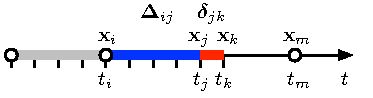
\includegraphics[width=0.6\textwidth]{figures/delta_time}
    \caption{The pre-integrated delta $\D_{ij}$ contains all motion from the last KF at time $i$, up to time $j$. 
    The current delta $\D_k$ contains the motion from times $j$ to $k$, computed from the last IMU measurement at time $k$.}
    \label{fig:delta_time}
\end{figure}

From all the considerations exposed above, the delta pre-integration algorithm is performed recursively via the following steps.

\paragraph{Initialization}
First, $\ol\D_{ii}$ is initialized to the null motion via the identity of the group, $\D_{\cE}$. 
Its covariance $\Cov_\Delta^{ii}$ and the Jacobian $\mjac{\D_{ii}}{\bfb_i}$ are set to zero. 

\paragraph{Calibration and retraction}
Second, at each reception of sensor data $\tilde\bfz_k$ at time $k$, we integrate during $\dt$ to obtain the delta corresponding to a single data sample
%
\begin{align}
    \bm\delta_k &= f(\tilde\bfz_k, \ol\bfb_i, \dt)  ~~~~~\in \cM, 
    \label{eq:data2delta}
\end{align}
%
using the calibration $\ol\bfb_i$ available in \keyframe\ $i$. 
In most cases, this function is split into the stages of data \textbf{calibration} $c()$, producing a vector in the tangent space, and \textbf{retraction} $\Exp()$, retracting 
it onto the manifold,
%
\begin{align}
    \bftau_k &= c(\tilde\bfz_k, \ol\bfb_i) \dt ~~~~~\in \Reals^{dim(\cM)}\\
    \bm\delta_k &= \Exp(\bftau_k) ~~~~~~~~\in \cM,
\end{align}
%
where the calibration, $c()$, depends on the sensor model, and the retraction, $\Exp()$, on the deltas Lie group.

\paragraph{Composition}
Third, this single delta is integrated onto the delta pre-integrated so far using the delta composition law
%
\begin{align}
    \ol\D_{ik} &= \ol\D_{ij} \circ \bm\delta_k ~~~~~\in \cM,
    \label{eq:deltaPlusDelta}
\end{align}
%
as can be seen in figure \figRef{fig:delta_time}.


\paragraph{Covariance and Jacobian}

The delta covariance, as well as the Jacobian of the pre-integrated delta with respect to the calibration parameters, are also pre-integrated using the chain rule and standard 
covariance propagation,
%
\begin{align}
    \Cov_\Delta^{ik} &= \mjac{\D_{ik}}{\D_{ij}}\Cov_\Delta^{ij}\mjac{\D_{ik}}{\D_{ij}}\tr 
    + \mjac{\D_{ik}}{\bm\delta_k}\mjac{\bm\delta_k}{\bfz_k}\Cov_\bfz\mjac{\bm\delta_k}{\bfz_k}\tr\mjac{\D_{ik}}{\bm\delta_k}\tr
    \\
    \mjac{\D_{ik}}{\bfb_i} &= \mjac{\D_{ik}}{\D_{ij}}\mjac{\D_{ij}}{\bfb_i} 
    + \mjac{\D_{ik}}{\bm\delta_k}\mjac{\bm\delta_k}{\bfb_i} ,
\end{align}
%
where $\mjac{\bm\delta_k}{\bfb_i}$, $\mjac{\bm\delta_k}{\bfz_k}$ are the Jacobians of \eqRef{eq:data2delta} and $\mjac{\D_{ik}}{\D_{ij}}$, $\mjac{\D_{ik}}{\bm\delta_k}$ the 
Jacobians of \eqRef{eq:deltaPlusDelta}, computed according to Lie theory \cite{sola2018micro}, to which we give a brief introduction in \secRef{sec:lie_groups}.



\bigskip

These steps are performed recursively until a new \keyframe\ is added to the factor graph. When it 
is the case, a motion factor is created as explained in the next section.


\subsection{Residual definition}
\label{sec:preint_residual}

When a new \keyframe\ is added to the problem at time $k=m$,
a factor is created to which we pass $\ol\D_{im}$, $\ol\bfb_i$,  $\mjac{\D_{im}}{\bfb_i}$, and $\Cov_\Delta^{im}$, with which the residual can be defined:
%
% The pre-integrated $\ol\D_{im}$ is used at the end of the pre-integration to define the residual:
%
\begin{align}
    \bfe_{im}(\bfx^i, \bfx^m, \bias^i) =  (\ol\D_{im} \oplus \mjac{\D_{im}}{\bfb_i}(\bfb_i-\ol\bfb_i) ) \ominus \hat\D_{im} 
    \label{eq:preint_residual}
\end{align}
%
with associated covariance $\Cov_\Delta^{im}$.
Here, $\bfb_i$ is the current  value of the sensor's calibration parameters,  $\hat\D_{im}=\bfx^m\boxminus\bfx^i$ is the expected delta between KFs, and $\{\op,\om\}$ are the 
 plus and minus operators described in section \secRef{sec:manifold_structure}. 
% That is, $\{\op,\om\}$ are $\{+,-\}$ for vectors, and for rotations we have $\bfR\op\bm\theta\te\bfR\Exp(\bm\theta)$ and $\bfR_2\om\bfR_1\te\Log(\bfR_1\tr\bfR_2)$. 
% The residual clearly depends on the KF states $\bfx^i,\bfx^m$ and the bias $\bfb_i$. It has an associated covariance  $\Cov_\Delta^{im}$.

In cases where the calibration parameters are subject to drift, the calibration drift is modeled as the integration of a random walk. This drift is included as a second factor 
in the factor graph, with residual error defined by
%
\begin{equation}
    \bfe^{\bias}_{im}(\bias^i, \bias^m) = \bias^m - \bias^i
\end{equation}
%
with associated covariance matrix
%
\begin{equation}
    \Cov_{\bias,im} = \bfW^c_{\bias} \Dt_{im}
\end{equation}


\subsection{Publishing the current optimal state}
\label{sec:publish-state}

Interestingly, the proposed algorithm allows for the publication, at the high rate of the motion sensor and with little lag, of the current state of the robot. 
To do so, we take advantage of the delta pre-integrated so far, which can be corrected in case we dispose of better estimates of the calibration parameters. 
The current state at time $t_k$ thus reads,
%
\begin{align}
    \bfx^k = \bfx^i \boxplus (\ol\D_{ik} \oplus \bfJ^{\D_{ik}}_{\bfb_i} (\bfb_i - \ol\bfb_i)).
\end{align}
%
This current state is optimal in the following sense. First, it uses the state $\bfx^i$ of the last \keyframe, which has been eventually optimized by the back-end. 
Second, it uses the most updated version of the calibration parameters $\bfb_i$ to correct the pre-integrated delta, thus minimizing the dead-reckoning drift of the motion 
increment from \keyframe\ time $t_i$ to the current time $t_k$.

The optimal state $\bfx^k$ is published at the rate of the motion sensor, which can reach the kHz, and might be used for closed-loop control of the robot. 
This is so regardless of the rate at which \keyframes\ are generated, and the rate at which the solver optimizes the problem. These rates, in any case, but especially 
if they are slow, will logically impact the accuracy of the published state.

%
%
%
%
\section{IMU pre-integration on Lie groups}
In this section, we will revisit the IMU pre-integration using the general pipeline defined in the previous section. First, we will frame the on-manifold pre-integration
of Forster \cite{forster2015imu, forster2017-TRO} as a delta pre-integration on a composite IMU delta group.
Second, we will present an alternative formulation of IMU pre-integration on a new compact delta matrix Lie group $\cD$ that we presented in \cite{fourmy2019absolute}.
We will finally discuss a few other alternatives.

\subsection{IMU pre-integraton on composite Lie group}
\label{sec:imu_preint_composite}

Let us come back to the IMU pre-integration problem, as stated by Forster \cite{lupton-09, forster2015imu}, defined in \secRef{sec:imu_preint_motivation}, and show that we 
can rewrite the algorithm in terms of the generalized pre-integration described in \secRef{sec:general-preint}.

The states involved in this integration are the base states $\bfx = [\posi{}{}, \bfv, \Rot{}{}]$ with deltas $\D=[\Dp,\Dv,\DR] \in \cM_{\D}$. 
The IMU produces biased and noisy measurements $\tilde\bfz = [\tilde\bfa, \tilde{\bfomega}]$ of the base proper acceleration and angular velocity, 
with bias $\bfb = [\bias_{a}, \bias_{\omega}]$ and noise $\noise = [\noise_{a}, \noise_{\omega}]$. 


\subsubsection{Definition of the deltas}

The IMU deltas, as introduced in \cite{lupton-09, forster2015imu} can be defined \cite{atchuthan-18-thesis} as the motion increments, in terms of position, velocity and orientation, 
between the current IMU frame and another frame, that started at the IMU state at time $i$, $\bfx_i=(\bfp_i,\bfv_i,\bfR_i)$, and that falls freely and without rotating at 
the acceleration of gravity (\figRef{fig:fff}).

\begin{figure}[t]
    \centering
    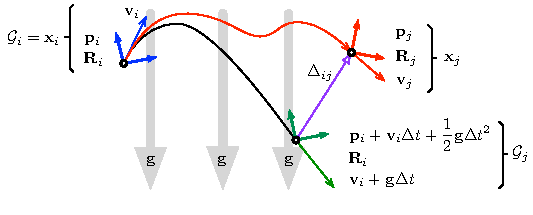
\includegraphics[width=0.8\textwidth]{figures/fff}
    \caption{The free-falling, non-rotating frame $\cG_t$ follows a parabolic trajectory governed only by gravity $\bfg$ and determined by the initial conditions 
    $\bfp_i$, $\bfv_i$ and $\bfR_i$ at time $i$ ($\cG_i=\bfx_i$, blue). The IMU delta $\D_{ij}$ between times $i$ and $j$ is defined as the state of the IMU at time 
    $j$ ($\bfx_j$, red) expressed in the free-falling frame at time $j$ ($\cG_j$, green).}
    \label{fig:fff}
\end{figure}

This derives in the definition of the operator $\boxminus$ in \eqRef{eq:boxminus} as what we detailed in \eqRef{eq:boxminus-forster}, and the operator 
$\boxplus$ in \eqRef{eq:boxplus} as being just its inverse.
% Then, $\bfx_k=\bfx_i\boxplus\D_{ik}$ is \cite[Eq.~32]{forster2017-TRO} and $\D_{ik}=\bfx_k\boxminus\bfx_i$ is \cite[Eq.~33]{forster2017-TRO}. 
Full details can be found in \cite[Section 3.4]{atchuthan-18-thesis}.


\subsubsection{Definition of the group operations}

Given two IMU deltas $\D=[\Dp,\Dv,\DR]$ and $\bfdelta=[\dpp,\dv,\dR]$, the group composition law $\D=\D\circ\bm\delta$ in \eqRef{eq:deltaPlusDelta} is defined as
%
\begin{equation} 
    \label{eq:composition_delta}
    \D \circ \bm\delta
    =
    \begin{bmatrix}
        \Dp + \Dv\dt + \DR\dpp \\
        \Dv + \DR\dv \\
        \DR\dR 
    \end{bmatrix}
\end{equation}
%
with a group identity element composed of the identity element of its Lie groups:
%
\begin{equation}
    \D_{\cE} = \begin{bmatrix}
    \bf0_3\\ \bf0_3\\ \bfI_3
    \end{bmatrix},
\end{equation}
%
the resulting inverse being
%
\begin{equation}
\label{eq:inverse_delta}
    \D^{-1} =     \begin{bmatrix}
    - \DR\tr(\Dp + \Dv \Dt) \\
    - \DR\tr \Dv \\
      \DR\tr
    \end{bmatrix}
\end{equation}
%
The calibration function $c()$ and exponential map $\Exp()$ are,
%
\begin{align}
    \bftau &= \begin{bmatrix}
    \bftau_a \\ \bftau_\omega
    \end{bmatrix} = \begin{bmatrix}
    \tilde\bfa-\bfb_a \\
    \tilde{\bfomega}-\bfb_\omega
    \end{bmatrix}\\
    \bfdelta &= \Exp(\bftau) = \begin{bmatrix}
    \frac12\bftau_a\dt^2 \\
    \bftau_a\dt \\
    \Exp(\bftau_\omega\dt)
    \end{bmatrix}
\end{align}
%
yielding $\bm\delta=f(\tilde\bfz,\bfb,\dt)$ in \eqRef{eq:data2delta} as
%
\begin{align}
    \bm\delta^k = \begin{bmatrix}
    \delta\bfp\\\delta\bfv\\\delta\bfR
    \end{bmatrix}^k =
    \begin{bmatrix}
    \tfrac12(\tilde\bfa-\bfb_a)\dt^2 \\
    (\tilde\bfa-\bfb_a)\dt \\
    \Exp((\tilde{\bfomega}-\bfb_\omega)\dt)
    \end{bmatrix}^k
    \label{eq:delta_function_forster}
\end{align}
%
% The pre-integration method in  \cite{forster2017-TRO} can be put in the general pre-integration formalism above by defining 
% $\bm\delta=f(\tilde\bfz,\bfb,\dt)$ in \eqRef{eq:data2delta} as:

\subsubsection{Delta pre-integration and factor residual}

The concatenation of the operations above lead exactly to the Forster's algorithm \cite{forster2017-TRO}:
%
\begin{itemize}
    \item Initialize $\D_{ii} = \D_\cE$, $\Sigma_\D=\bf0$, $\bfJ^\D_\bfb = \bf0$, and $\ol\bfb_i = \bfb_i$.
    \item Calibrate data and retract to manifold using \eqRef{eq:delta_function_forster}.
    \item Compose $\ol\D$ using \eqRef{eq:composition_delta}.
\end{itemize}
%
Likewise, the factor residual is computed following \secRef{sec:preint_residual} exactly.



\subsection{IMU pre-integration on compact Lie group}
\label{sec:imu_preint_compact}

This formulation was proposed in our published paper \cite{fourmy2019absolute}.

\subsubsection{Delta definition}

We propose a matrix form of the Lie group of IMU deltas as,
%
\begin{align}\label{eq:delta_Lie}
    \D &= 
    \begin{bmatrix}
    \DR & \Dv & \Dp \\
    \bf0 & 1 & \Dt \\
    \bf0 & 0 & 1
    \end{bmatrix} \in \cD \subset \bbR^{5\times 5}
    ~.
\end{align}
%
The three main constituents of such deltas, namely $\Dp$, $\Dv$, and $\DR$, are defined exactly as in the composite case above. 
Being computed in the same manner, the definition of the $\boxminus$ and $\boxplus$ operators is a trivial manner of forming the matrix deltas from 
\eqRef{eq:boxminus-forster}, yielding proper expressions for
%
\begin{align*}
\hat\D_{im} &= \bfx_m \boxminus \bfx_i &
\bfx_m &= \bfx_i \boxplus \hat\D_{im}.
\end{align*}
%
Notice a fourth, time interval component $\Dt$ as being also part of the delta definition.

\subsubsection{Group operations}
Group composition, identity, and inverse stem from regular matrix product, identity, and inverse (with $\DR\inv=\DR\tr$),
%
\begin{align}
    \D\circ\bm\delta 
    &= 
    \begin{bmatrix}
    \DR\dR & \Dv + \DR\dv & \Dp+\Dv\dt + \DR\dpp \\
    \bf0 & 1 & \Dt+\dt \\
    \bf0 & 0 & 1
    \end{bmatrix}
    \label{eq:compact_composition}
    \\
    \D_\cE&=\begin{bmatrix}
    \bfI_3 & \bf0 & \bf0 \\
    \bf0 & 1 & 0 \\
    \bf0 & 0 & 1 
    \end{bmatrix} = \bfI_{5\times5}
    \label{eq:identity}
    \\
    \D\inv &= \begin{bmatrix}
    \DR\tr & -\DR\tr\Dv & -\DR\tr(\Dp-\Dv\Dt) \\
    \bf0 & 1 & -\Dt \\
    \bf0 & 0 & 1
    \end{bmatrix} ~.
    \label{eq:inverse}
\end{align}
%
Comparing against \eqsRef{eq:composition_delta}{eq:inverse_delta} we observe that this matrix Lie group behaves equivalently to Forster's IMU deltas above.


\subsubsection{Lie algebra \texorpdfstring{$\mathfrak{d}$}{d} and exponential map}

The compact Lie group defines a different Lie algebra parametrization than Forster's, and therefore a different exponential map.
The Lie algebra elements $\bftau\hhat$ and their isomorphic Cartesian $\bftau$ have the forms
%
\begin{align}
    \label{eq:lie_algebra}
    \bftau\hhat &= \begin{bmatrix}
    \hatx{\bth} & \bfrho & \bfupsilon \\
    \bf0 & 0 & \Dt \\
    \bf0 & 0 & 0
    \end{bmatrix} ~~~\in \mathfrak{d}
    ,&
    \bftau &= \begin{bmatrix}
    \bfrho \\ \bfupsilon \\ \bth \\ \Dt
    \end{bmatrix}
    \te \Dt \begin{bmatrix}
    \bfv \\ \bfa \\ \bw \\ 1
    \end{bmatrix} 
    ~~~\in \bbR^{10}
    ,
\end{align}
%
with $\bfv\te\dot\Dp$, $\bfa\te\dot\Dv$ and $\hatx{\bw}\te\DR\tr\dot\DR$.
Operators $\wedge$ and $\vee$ are defined so that $\bftau\hhat=(\bftau)\hhat$ and $\bftau=(\bftau\hhat)\vvee$.

The exponential map transfers tangent elements to the group; the logarithmic map is its inverse,
%
\begin{align}
    \D &= \Exp(\bftau) \te \exp(\bftau\hhat) = \begin{bmatrix}
    \Exp(\bth) & \bfQ\bfupsilon & \bfQ\bfrho+\bfP\bfupsilon\Dt \\
    \bf0 & 1 & \Dt \\
    \bf0 & 0 & 1
    \end{bmatrix} %\in\cD 
    \label{eq:compact_exp}
    \\
    \bftau &= \Log(\D) \te \log(\D)\vvee = \begin{bmatrix}
    \bfQ\inv(\Dp-\bfP\bfQ\inv\Dv\Dt) \\
    \bfQ\inv\Dv \\
    \Log(\DR) \\
    \Dt 
    \end{bmatrix} %\in \bbR^{10}
    \label{eq:compact_log}
\end{align}
%
where $\Log()$ is obtained by identifying terms in \eqRef{eq:delta_Lie} and \eqRef{eq:compact_exp}.
Matrices $\bfP$ and $\bfQ$ are provided in the appendix's \secRef{sec:IMULieGroup}.


\paragraph{The case of IMU data, leading to \texorpdfstring{$\bfv=0$}{bfv=0}}
\label{sec:IMU_case}

We showed that IMU deltas could be interpreted as the motion relative to the free-falling frame (\figRef{fig:fff}), which has initial velocity $\bfv_i$, and the same physical analogy applies to the compact Lie group.
Thus the tangent velocity $\bfv=\dot\Dp$  is zero at the start of the integration step. 
%
Since the exponential $\Exp(\bm\nu\Dt)$ assumes a constant tangent vector $\bm\nu=(\bfv,\bfa,\bw,1)$ during the interval $\Dt$, we have that $\bfv=0$ during the full step. 
%
This gives immediately
%
\begin{equation}
    % \D &= 
    \Exp\left(\begin{bmatrix}
    \bf0 \\ \bfa \\ \bw \\ 1
    % \hatx{\bw} & \bfa & \bf0 \\
    % \bf0 & 0 & 1 \\
    % \bf0 & 0 & 0 
    \end{bmatrix}\Dt\right) 
    = \begin{bmatrix}
    \Exp(\bw\Dt) & ~\bfQ\bfa\Dt~ & \bfP\bfa\Dt^2 \\
    \bf0 & 1 & \Dt \\
    \bf0 & 0 & 1
    \end{bmatrix}
    ~,
    \label{eq:exp_compact_imu}
\end{equation}
%
which we will use to integrate IMU data.






%
%
%
\subsubsection{Pre-integration pipeline}
\label{sec:pre-integration-pipeline}

Here we recall the general pre-integration pipeline in the case of the compact Lie group, pointing at the minor differences with the composite Lie group case.
The following pipeline of operations is performed to recursively pre-integrate IMU data into a unique measurement.

\paragraph{Initialization}
Pre-integration starts after each \keyframe\ with $\ol\D_{ii} = \bfI$, $\bfSigma^\Delta_{ii} = \bf0$ and $\mjac{\D_{ii}}{\bfb} = \bf0$, using $\ol\bfb_i = \bfb_i$ the current best estimate of the bias at time $i$.

\paragraph{Calibration}
At the reception of each IMU measurement $\bfz_k=(\bfa,\angvel{}{})_k$, start by correcting it with available  bias estimates $\ol\bfb_i=(\bias_a,\bias_{\omega})_i$, 
to produce the tangent vector $\bftau=\bm\nu\dt$. For this, set the velocity part of $\bm\nu$ to zero as the IMU is by definition at zero speed \wrt 
the moving frame, as in \eqRef{eq:exp_compact_imu}. Obtain at the same time the respective Jacobians,
%
\begin{align}
    \bftau_k &= 
    \begin{bsmallmatrix}
    \bf0 \\ \bfa - \bias_a \\ \bw - \bias_{\omega} \\ 1
    \end{bsmallmatrix}\dt, 
    &
    \mjac{\bftau}{\bfz} &= 
    \begin{bsmallmatrix}
    \bf0 & \bf0 \\
    \bfI & \bf0 \\
    \bf0 & \bfI \\
    0 & 0
    \end{bsmallmatrix}\dt,
    &
    \mjac{\bftau}{\bfb} &= 
    -\begin{bsmallmatrix}
    \bf0 & \bf0 \\
    \bfI & \bf0 \\
    \bf0 & \bfI \\
    0 & 0
    \end{bsmallmatrix}\dt 
    \label{eq:preint_debiasing}
\end{align}
%
\paragraph{Retraction}
Second, use the exponential map \eqRef{eq:exp_compact_imu} to obtain the current delta step $\bm\delta^k$ in the group manifold, and obtain Jacobian
%
\begin{align}
    \bm\delta^k &= \Exp(\bftau_{k})~,
    &
    \mjac{\bm\delta}{\bftau} &= \mjac{}{r}(\bftau_k)
    ~.
\end{align}

\paragraph{Composition}
Third, use group composition \eqRef{eq:compact_composition} to update the pre-integrated delta; obtain Jacobians
%
\begin{align}
    \ol\D_{ik} &= \ol\D_{ij}\circ\bm\delta^k ~,
    &
    \mjac{\D_{ik}}{\D_{ij}} &= \Ad{\bm\delta^k}\inv
    ~,&
    \mjac{\D_{ik}}{\bm\delta^k} = \bfI
    \label{eq:pre_composition}
    ~,
\end{align}
%
where $\Ad{\bm\delta}$ is the adjoint and $\mjac{}{r}$ is the right Jacobian ---see appendices \secRef{sec:imu_compact_adjoint}, \secRef{sec:imu_compact_right_jacobian} and technical paper \cite{sola2018micro} for reference. 

\paragraph{Covariance}
Fourth, propagate the delta covariance
%
\begin{align}
    \bfSigma^\Delta_{ik} &= \mjac{\D_{ik}}{\D_{ij}}\bfSigma^\Delta_{ij}\mjac{\D_{ik}}{\D_{ij}}\tr 
    + \mjac{\D_{ik}}{\bfz}\bfSigma_\bfz\mjac{\D_{ik}}{\bfz}\tr
    ~,
\end{align}    
%
with $\bfSigma_\bfz$ the covariance of the IMU measurements $\bfz$, and $\mjac{\D_{ik}}{\bfz}=\mjac{\D_{ik}}{\bm\delta}\mjac{\bm\delta}{\bftau}\mjac{\bftau}{\bfz}$ computed using the chain rule. 

\paragraph{Jacobian}
Finally, integrate the Jacobian of the delta \wrt the biases
%
\begin{align}
    \mjac{\D_{ik}}{\bfb} &= \mjac{\D_{ik}}{\D_{ij}}\mjac{\D_{ij}}{\bfb} 
    + \mjac{\D_{ik}}{\bm\delta^k}\mjac{\bm\delta}{\bftau}\mjac{\bftau}{\bfb}
    ~.
\end{align}
%

\bigskip

Pre-integration is complete (\figRef{fig:delta_time}) when $k=m$, which yields $\ol\D_{im}$, $\bfSigma^\Delta_{im}$ and $\mjac{\D_{im}}{\bfb}$.


\subsubsection{Factor residual}
Computation of the residual in the case of the Lie Delta group formulation follows the steps defined in \secRef{sec:general-preint}.
% However, since the Delta is directly defined as a Lie group, the formulation is actually simplified because  ... 
Use the pre-integrated Jacobian $\mjac{\D_{im}}{\bfb}$ to correct the pre-integrated delta $\ol\D_{im}$ to account for the new bias estimate $\bfb_i\neq\ol\bfb_i$,

\begin{align}
    \D_{im}(\bfb_i) &= \ol\D_{im}\oplus\mjac{\D_{im}}{\bfb}(\bfb_i-\ol\bfb_i) 
    ~.
\end{align}
%
Use \eqRef{eq:boxminus-forster} as $\boxminus$ to compute the expected delta from  $\bfx_i$ to $\bfx_m$,
%
\begin{align}
    \widehat\D_{im}(\bfx_i,\bfx_m) &= \bfx_m \boxminus \bfx_i 
    ~.
\end{align}
%
Compute the residual in the  tangent of $\cD$ at $\D_{im}$,
%
\begin{align}
    \bfe^\D_{im}(\bfx_i,\bfx_m,\bfb_i) 
    &=\widehat\D_{im}(\bfx_i,\bfx_m) \ominus \D_{im}(\bfb_i) \\
    &=\Log(\D_{im}(\bfb_i)\inv \circ \widehat\D_{im}(\bfx_i,\bfx_m)) \in \bbR^9
~,
\end{align}
%
%and drop the $\Dt$ part from the residual after the $\Log()$ ---see comment in \secRef{sec:uncertainty}.
In this last equation, the minus operator $\ominus$ is the lift operator defined in \eqRef{eq:retract_lift} and specialized for this particular group.

\subsubsection{Jacobians, uncertainty}
\label{sec:uncertainty}

For general functions $f:\cM\to\cN;y=f(x)$, we propagate uncertainty normally via the Jacobians 
$\mjac{y}{x}\te\dpar{y}{x}$, \ie, $\Cov_y=\mjac{y}{x}\,\Cov_x\,\mjac{y}{x}\tr$. 
These Jacobians map the tangent spaces of the manifolds $\cM,\cN$ at $x$ and $y$, and in the case of vector spaces, they resort to the classical Jacobian.
They also satisfy the chain rule, which we use extensively in our developments.
Ample reference and justification of this approach can be found in \cite{sola2018micro}.

A comment is however necessary for the present IMU case.
It relates to the uncertainty of the last component of the tangent space \eqRef{eq:lie_algebra}, which is the time $\Dt$. This component has no uncertainty by definition. 
Having it in the covariances would imply singularity and result in the risk of several well-known numerical issues. 
We therefore systematically marginalize this time component out of the covariances, simply by removing the last row and column. 


\subsection{About the choice of the proper Lie group}

\subsubsection{Our IMU Lie group versus Forster's method}

Mathematically, and disregarding methodology, the main difference between our method (\secRef{sec:imu_preint_composite}) and Forster's \cite{forster2017-TRO} (\secRef{sec:imu_preint_compact}) is to be found in the exponential map. 
To see it, let us consider small rotation increments $\bth=\bw\dt$ captured at each single IMU sample. 
In such cases, the matrices $\bfP,\bfQ$ appearing in the exponential map \eqRef{eq:compact_exp} and detailed in \eqRef{eq:RQP} can be approximated by $\bfP\approx\tfrac12\bfI$ and $\bfQ\approx\bfI$.
The exponential becomes,
%
\begin{align}
    \Exp\left(\begin{bmatrix}
    \bf0 \\ \bfa \\ \bw \\ 1
    \end{bmatrix}\dt\right) \approx \begin{bmatrix}
    \Exp(\bw\dt) & \bfa\dt & \tfrac12\bfa\dt^2 \\
    \bf0 & 1 & \dt \\
    \bf0 & 0 & 1
    \end{bmatrix}
~,
\end{align}
%
where we find the terms $\bfa\dt$ and $\tfrac12\bfa\dt^2$, which are exactly the terms obtained with Forster's method \eqRef{eq:delta_function_forster}. 
In effect, with this approximation, if we now compact all the steps \eqsRef{eq:preint_debiasing}{eq:pre_composition} of our integration into a cumulative expression,
%
\begin{align}
    \D_{ik} = \prod_{j=i+1}^k \Exp\left(\begin{bmatrix}
    \bf0 \\ (\bias_a^i - \bias_a^j) \\ (\bias_{\angvel{}{}}^j-\bias_{\angvel{}{}}^j) \\ 1
    \end{bmatrix}\dt\right)
~,
\end{align}
%
it is possible (although tedious) to show that both Forster's and our method are exactly equivalent when $\bw\dt\to0$.
% , which is usually a valid hypothesis.
% These differences should not constitute an argument against Forster, since in practice we typically have extremely small steps $\bw\dt$ and the approximation holds very well.



\subsubsection{Further discussion regarding Lie group choice}

Regarding "compact group" designs, there is still another proposal, the $\SE_2(3)$ group proposed by \cite{barrau2020mathematical, brossard2021associating}, 
which can be used for IMU pre-integration. This proposal differs from ours in the following aspects:

\begin{itemize}
    \item The $\SE_2(3)$ group does not contain the time and therefore the composition law does not account for the whole integration. Some extra algebra needs to be added.
    \item The $\SE_2(3)$ group is easier to manipulate since the closed forms for the exponential map, the adjoint, and the right-Jacobian are easier to obtain.
    \item Our group better separates between the delta states and the velocity of these states which depend only on the IMU data.
\end{itemize}

Therefore, it is apparent that depending on the structure of the defined Lie group, we can have different designs:
\begin{itemize}
    \item Forster \cite{forster2015imu}: Composite Lie group
    \item Barrau \cite{barrau2020mathematical}: $\SE_2(3)$ compact Lie group without time
    \item Fourmy \cite{fourmy2019absolute}: Compact IMU group with time
\end{itemize}

In the context of filtering, using a compact group formulation of the robot state has been proven to improve greatly the basin of convergence of the so-called
Invariant Kalman Filter \cite{barrau2018invariant, hartley2020contact}. This method tackles one of the issues of standard EKF: 
the Jacobians are computed around the current estimates, which leads to an inconsistency of the estimate if the filter is initialized far from the optimal. 
However, this issue is not so present with factor graph optimization since we repeatedly linearize around the new estimates.
Nevertheless, it seems that compact Lie groups may provide slightly better performances than composite Lie groups \cite{brossard2021associating}, thanks 
to a more precise linearization \wrt\ the IMU biases and a covariance propagation that better represents the geometry of the problem.

However one may ask whether these more elegant mathematical formulations and slight improvements are worth the effort. Compact designs may be seen as going against
our modularity philosophy since for each new motion sensor, we need to find a new appropriate Lie group instead of being able to reuse the machinery developed
for composite groups, which is vastly simpler.




\section{Related works}

Pre-integration principles were laid out by Lupton \cite{lupton-09} for a smoothing-based visual-inertial estimator. His work was motivated partly 
by the fact that previous systems required a precise initialization of orientation and velocity (using a specialized routine) to begin to integrate IMU measurements. 
With this new formulation, Lupton noted that pre-integration of IMU data permitted the use of measurements immediately and delay the estimation of the initial 
orientation about the gravity vector in particular. 

This seminal work was quickly adopted by other authors using smoothing filters \cite{carlone2014eliminating}. As pioneering as this work was, it was however 
limited by the use of Euler angles whose problematic geometric properties are notorious. Indelman \cite{Indelman-2013-7768} first proposed to use the exponential of the 
matrix rotation group instead of Euler integration and to relax the assumptions of non-rotating and flat earth of Lupton \cite{lupton-09}. Forster \cite{forster2015imu, forster2017-TRO}
proposed the same formulation using the SO(3) Lie group, which was adapted to the quaternions group S$^3$ by Atchuthan \cite{atchuthan-18-thesis}. Various experiments brought to light three main problems with the Euler angle formulation, that are completely absent 
from the quaternion "on-manifold" formulation. Firstly, first-order integration of angular velocities using Euler angles is approximate, which leads to accumulated errors 
for high angular velocities or sampling rate. Secondly, the log-likelihood of the angular displacement is not invariant under the action of rigid body transformations, 
\eg the choice of the world frame influence the results of the estimation. Finally, the well-known gimbal lock singularity of Euler angles has a consequence 
on the IMU noise covariance propagation, which is severely degraded when the robot trajectory comes close to the singularity. 
\cite{shen2015tightly}, later improved in \cite{qin2018vins} proposed to use a more precise numerical integration procedure than the default forward Euler used by Forster. 
Eckenhoff \cite{eckenhoff2019closed} derived closed-form solutions of the pre-integration equations using various piecewise constant models.

Barrau \cite{barrau2020mathematical} described a compact matrix Lie group for the propagation of pre-integration errors taking into account the earth rotation with the aerospace
inertial navigation system in view. This work was later extended \cite{brossard2021associating} and showed that the linearized bias update is slightly more precise than 
the work of Forster \cite{forster2017-TRO}. Le Gentil \cite{le2020gaussian} used a different trajectory parametrization framework by formulating the pre-integration algorithm 
in the context of Gaussian Process smoothing. Self-calibration of IMU/Camera time offsets was also developed \cite{yang2020analytic}. 
\cite{luo2021unified} derived a comprehensive collection of motion models depending on the various possible choices of reference frames and motion conditions. 

As we saw the pre-integration theory began in the context of visual-inertial odometry. It was however adapted to other high rate sensors such as wheel odometry \cite{quan2019tightly}, 
possibly including self-calibration \cite{deray-19-selfcalib}. In his thesis, Atchuthan (\cite[Section 4.3]{atchuthan-18-thesis}) derived the general form of the pre-integration 
equations as a sensor agnostic form that is integrated in the state estimation framework WOLF \cite{sola2021wolf}. As previously mentioned, other teams applied pre-integration theory in the 
context of factor graph legged robots state estimation to derive new leg-odometry factors \cite{hartley2018legged, wisth2019robust, wisth2020preintegrated}.
It was also applied to integrate drone dynamics to estimate external forces disturbances \cite{nisar2019vimo}.

In \chpRef{chp:underactuade_dynamics}, we propose to pre-integrate force-torque measurements that are present in some legged-robots. 
We show that permits to estimate the centroidal quantities of the robot as well making the kinematic bias on the center of mass measurements observable. 
A practical implementation is demonstrated in \chpRef{chp:centroidal_estimation}, which is based on our paper \cite{fourmy2021contact}



\section{Conclusion}

In this chapter, we have recalled the mathematics of the pre-integration,
which is very important when handling high-frequency measurements strongly
correlated with Lie-group quantities. Pre-integration was first introduced for
handling IMU in the MAP framework, as we also did in our experiments. We
introduced here a reformulation of the original mathematics, which lead to
minor practical differences, but mostly allows us to more systematically generalize
to other measurements. We also believe that this formulation, relying on
Lie theory, gives some easier intuition to catch, at least when the reader is
familiar with Lie groups.

We are now going to use this formulation to handle force sensors, which also
stream meaningful information at high (1kHz) frequency, and integrate to
to an extended MAP problem where the centroidal quantities are also estimated
simultaneously to previously estimated basis state and map variables.
